\subsection{User Interfaces}
\begin{figure}[H]
	\centering
	\begin{subfigure}[b]{0.4\textwidth}	
		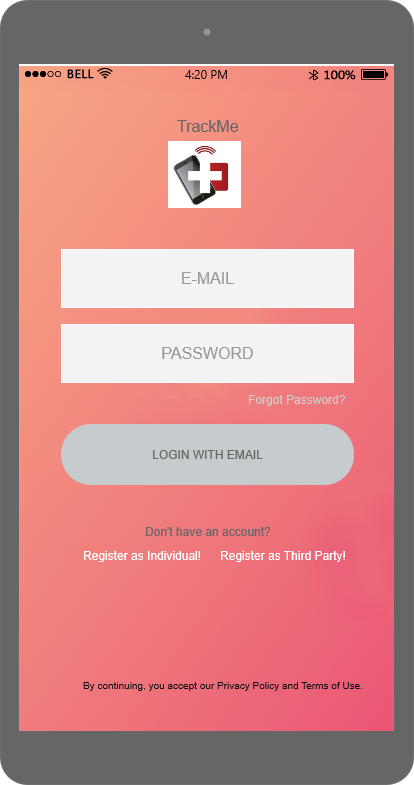
\includegraphics[width=4cm,height=7cm]		{./Mockups/1_Login.png}
      	\caption{Login for TrackMe}
        \label{TrackMe_login}
	 \end{subfigure}
\end{figure}
This is the login page where a user of type individual or third party can login by entering their credentials. If a user is new then they can register as individual or third party depending on their category.
\newline\newline\newline\newline
\textbf{Data4Help}
\newline\qquad{1. User Type: Individual}

\begin{figure}[H]
	\centering
	\begin{subfigure}[b]{0.4\textwidth}	
		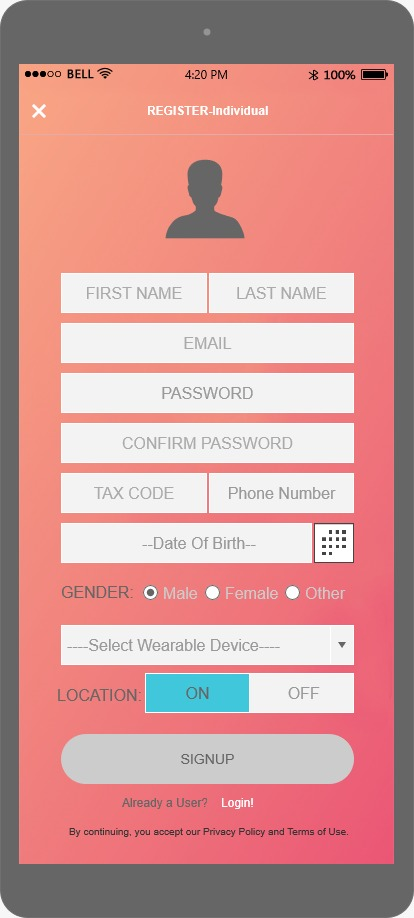
\includegraphics[width=4cm,height=7cm]		{./Mockups/2_I-Register.jpeg}
      	\caption{Registration for individuals}
        \label{TrackMe_register1}
	 \end{subfigure}
\end{figure}

The individual can check their vitals, and get to know about the third parties accessing their data and can receive the request of the third party which they can accept/reject when the third party asks the data about a specific individual.

\begin{figure}[H]
	\centering
	\begin{subfigure}[b]{0.3\textwidth}	
		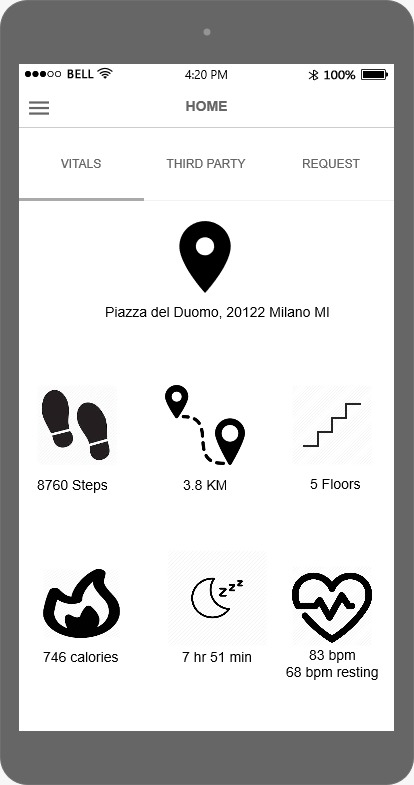
\includegraphics[width=4cm,height=7cm]		{./Mockups/3_I-Home.jpeg}
      	\caption{Individual Checks Vitals}
        \label{TrackMe_vitals}
	 \end{subfigure}
     \begin{subfigure}[b]{0.3\textwidth}	
		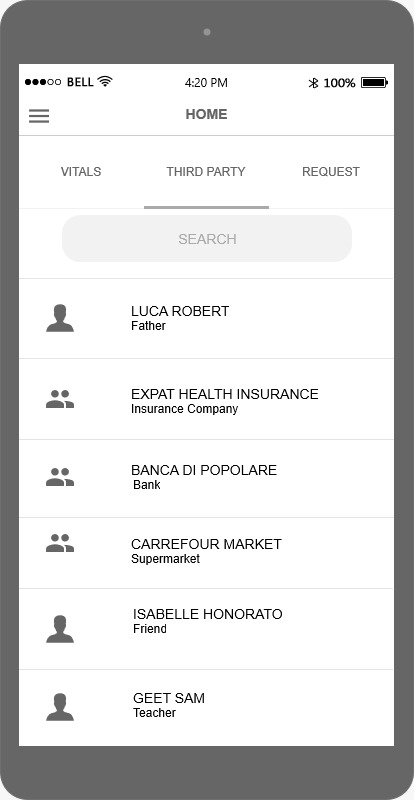
\includegraphics[width=4cm,height=7cm]		{./Mockups/4_I-DetailsOfThirdParty.jpeg}
      	\caption{Third party accessing individual's data}
        \label{TrackMe_3party}
	 \end{subfigure}
     \begin{subfigure}[b]{0.3\textwidth}	
		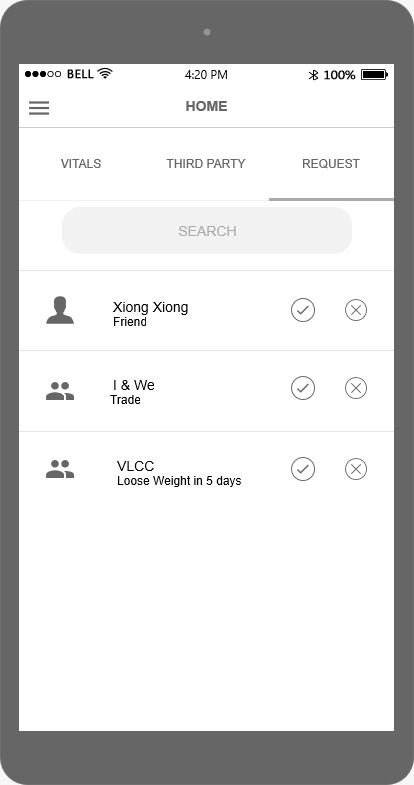
\includegraphics[width=4cm,height=7cm]		{./Mockups/5_I-Request.jpeg}
      	\caption{Accept/Reject access request}
        \label{TrackMe_acerej}
	 \end{subfigure}
\end{figure}

2. User Type: 3rd Party

\begin{figure}[H]
	\centering
	\begin{subfigure}[b]{0.4\textwidth}	
		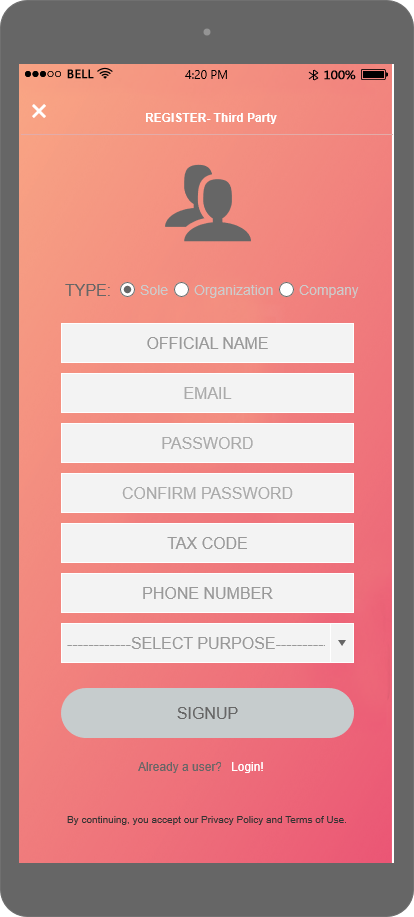
\includegraphics[width=4cm,height=7cm]		{./Mockups/2_T-Register.png}
      	\caption{Registration for Third Party}
        \label{TrackMe_register2}
	 \end{subfigure}
\end{figure}

Third party can check individual's or group of individual's data, make new requests for specific individual's data and group of individual's data, and view the status of earlier requests made to know whether they are requested, accepted or pending.

\begin{figure}[H]
	\centering
	\begin{subfigure}[b]{0.4\textwidth}	
		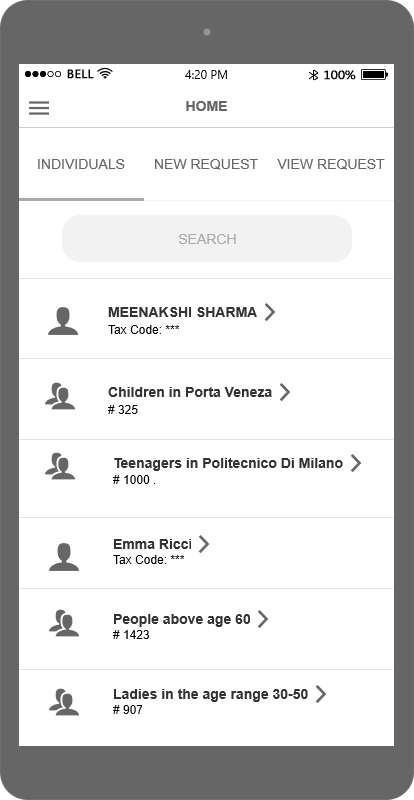
\includegraphics[width=4cm,height=7cm]		{./Mockups/3_T-Home.png}
      	\caption{Access individual's data}
        \label{TrackMe_data}
	 \end{subfigure}
     \begin{subfigure}[b]{0.4\textwidth}	
		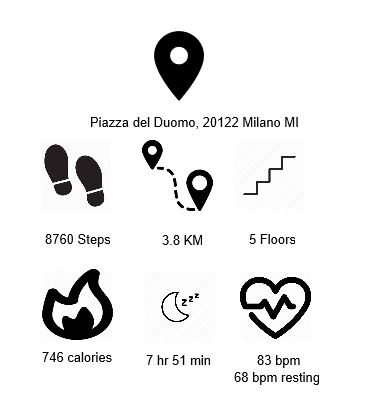
\includegraphics[width=\textwidth]		{./Mockups/3_T_popup.jpg}
      	\caption{This Popup appears on the screen on clicking on specific individual's list and for group of individuals another list of all individuals appears with their vitals.}
        \label{TrackMe_popup}
	 \end{subfigure}
\end{figure}

\begin{figure}[H]
	\centering
     \begin{subfigure}[b]{0.4\textwidth}	
		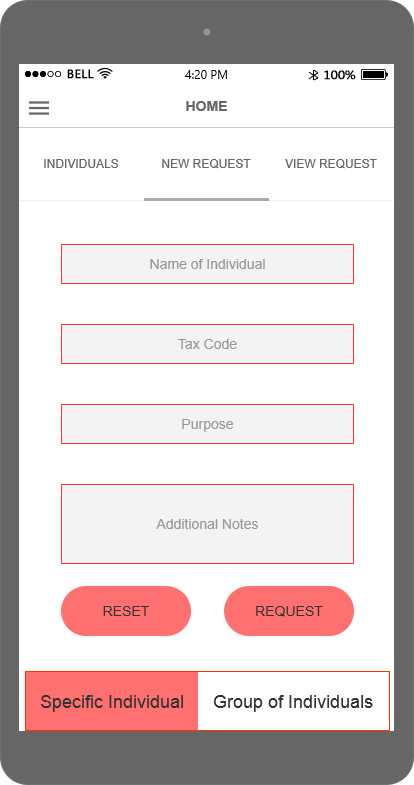
\includegraphics[width=4cm,height=7cm]		{./Mockups/4_T_1-NewRequest.png}
      	\caption{Make new request for individual}
        \label{TrackMe_reqind}
	 \end{subfigure}
     \begin{subfigure}[b]{0.4\textwidth}	
		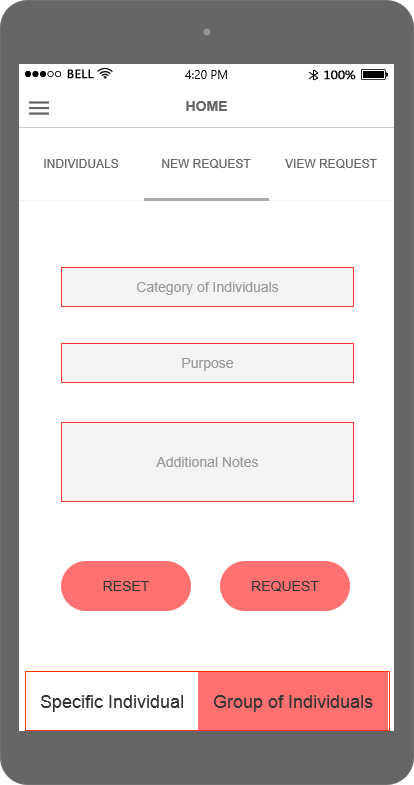
\includegraphics[width=4cm,height=7cm]		{./Mockups/4_T_2-NewRequest.png}
      	\caption{Make new request for Group of Individuals}
        \label{TrackMe_reqgroup}
	 \end{subfigure}
     \begin{subfigure}[b]{0.4\textwidth}	
		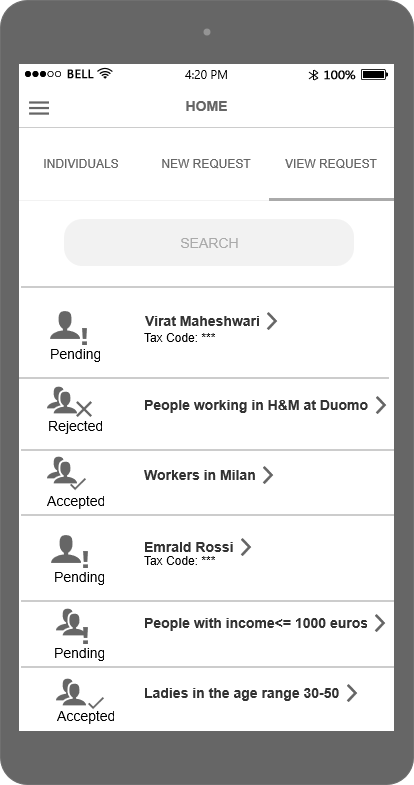
\includegraphics[width=4cm,height=7cm]		{./Mockups/5_T-ViewRequest.png}
      	\caption{View Requests}
        \label{TrackMe_viewreq}
	 \end{subfigure}
\end{figure}
.
\newline\newline\newline\newline\newline\newline\newline\newline
\textbf{Menu}
\newline
This includes all the extra features which is offered to the users. The menu remains same for both type of users: individual or third party.

\begin{figure}[H]
	\centering
	\begin{subfigure}[b]{0.4\textwidth}	
		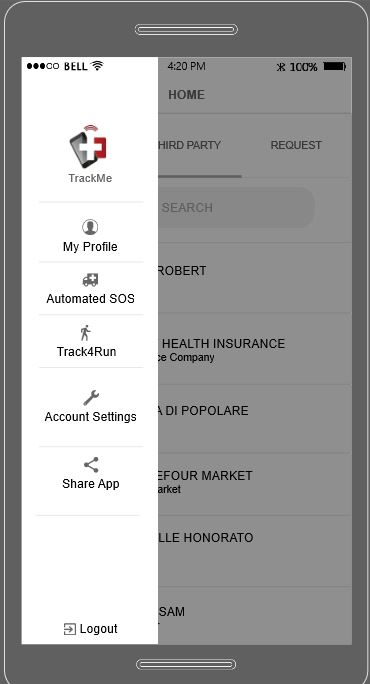
\includegraphics[width=4cm,height=7cm]		{./Mockups/6_Menu.JPG}
      	\caption{Menu}
        \label{TrackMe_Menu}
	 \end{subfigure}
\end{figure}

Menu-1. My Profile\newline
User can update their data in MyProfile section.

\begin{figure}[H]
	\centering
	\begin{subfigure}[b]{0.4\textwidth}	
		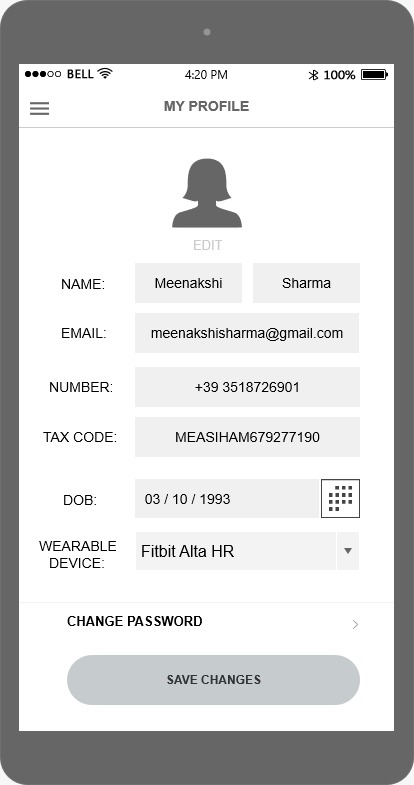
\includegraphics[width=4cm,height=7cm]		{./Mockups/7_I-MyProfile.jpeg}
      	\caption{Individual-MyProfile}
        \label{TrackMe_indpro}
	 \end{subfigure}
     \begin{subfigure}[b]{0.4\textwidth}	
		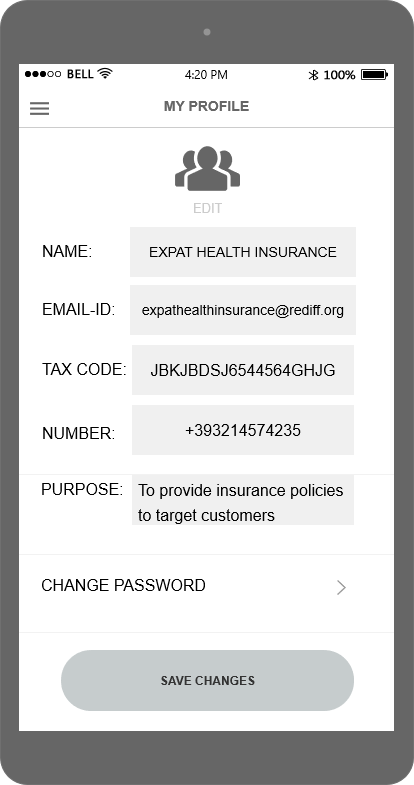
\includegraphics[width=4cm,height=7cm]		{./Mockups/7_T-MyProfile.png}
      	\caption{3rd Party-MyProfile}
        \label{TrackMe_3ppro}
	 \end{subfigure}
\end{figure}

.\newline\newline
Menu-2. AutomatedSOS\newline
This is only for individuals .\newline If they have not registered tot his service then they will be directed to the payment page where they can pay and register for the service.\newline If they have registered to this service, then they see a map with nearby hospitals and pharmacies.\newline In case of emergencies, they can track ambulance in the map.

\begin{figure}[H]
	\centering
	\begin{subfigure}[b]{0.4\textwidth}	
		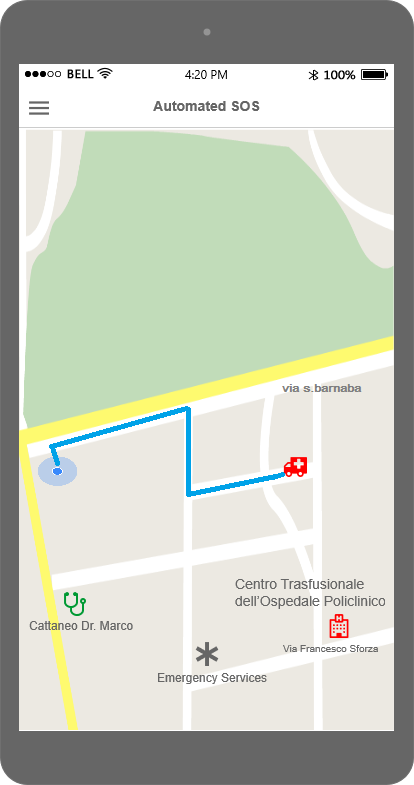
\includegraphics[width=4cm,height=7cm]		{./Mockups/8_I-AutomatedSOS.png}
      	\caption{AutomatedSOS}
        \label{TrackMe_AutomatedSOS}
	 \end{subfigure}
\end{figure}

Menu-3. Track4Run\newline
This service is for both the users, individual and third party.\newline If the user has not upgraded to this service, then for individual who can be an athlete or a spectator and the third party who can be a spectator will be directed to a payment page to pay and use the service.\newline The third party organizer who has not registered will be directed to a form and then a payment page. The organizer defines the path, theme of race and other details of the race in the form.\newline If the user has registered, then they will see a live map with all the position of the athletes.

\begin{figure}[H]
	\centering
	\begin{subfigure}[b]{0.4\textwidth}	
		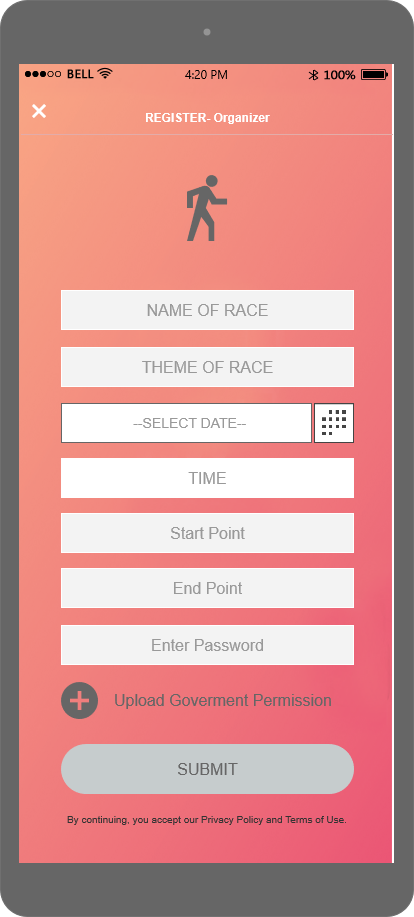
\includegraphics[width=4cm,height=7cm]		{./Mockups/9_T-Oragnizer.png}
      	\caption{Organizer form}
        \label{TrackMe_org}
	 \end{subfigure}
     \begin{subfigure}[b]{0.4\textwidth}	
		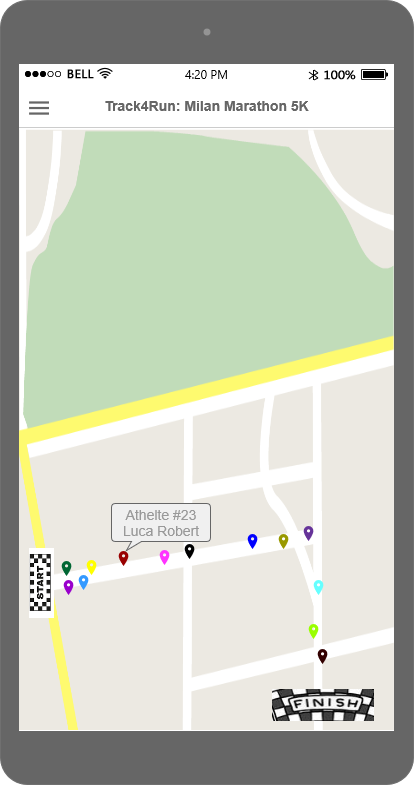
\includegraphics[width=4cm,height=7cm]		{./Mockups/9-Track4Run.png}
      	\caption{Track4Run}
        \label{TrackMe_Track4Run}
	 \end{subfigure}
\end{figure}

\textbf{Mobile Application for Ambulance Drivers}
This is an application made explicitly for Ambulance where they receive request in form of push notification and they accept it and the first driver to accept is navigates to the individual's location.

\begin{figure}[H]
	\centering
	\begin{subfigure}[b]{0.4\textwidth}	
		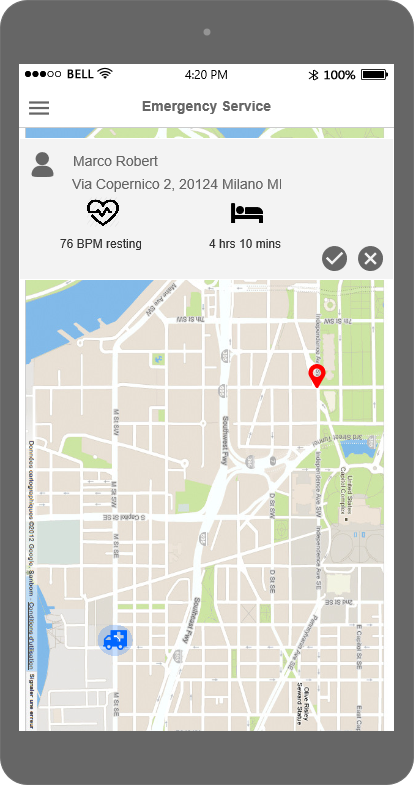
\includegraphics[width=4cm,height=7cm]		{./Mockups/1-Ambulance.png}
      	\caption{Accept Request}
        \label{TrackMe_ambulance}
	 \end{subfigure}
     \begin{subfigure}[b]{0.4\textwidth}	
		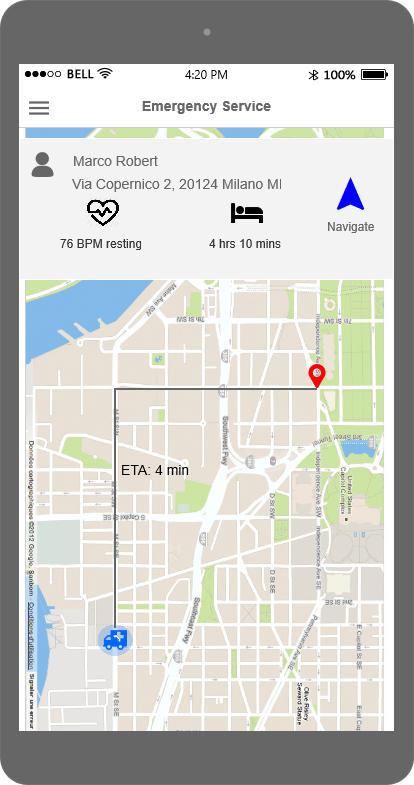
\includegraphics[width=4cm,height=7cm]		{./Mockups/2-Ambulance.png}
      	\caption{Navigate}
        \label{TrackMe_navigate}
	 \end{subfigure}
\end{figure}
.\newline\newline

\subsection{Software Interfaces}
\begin{enumerate}
\item \textbf{Data4Help API}
\newline \qquad TrackMe extracts location and health of the individual from the API of the   wearable device and stores it in a database. An API of the database is created which is provided to the other services of TrackMe. This information is used for many purposes. “AutomatedSOS” and “Track4Run” uses the API of the “Data4Help” in order to provide their service. Both the services exploit the services of “Data4Help”. “AutomatedSOS” uses the API to monitor the health status of elderly people and help them by providing an ambulance. “Track4Run” uses the API to extract the location and health of individuals registered as athletes. The location will be displayed to all the users and the health status of athletes will be monitored by the third party organizers.
\item \textbf{Ambulance Application}
\newline\qquad TrackMe develops an application for all the ambulance drivers associated with major Hospitals in the city of Milan. The application fetches the details and location of all the ambulance driver. When the health status of an subscribed individual is below a threshold value, the software sends a push notification to the nearby ambulance drivers phone with the details and location of the individual. Once an ambulance driver accept the request, the software removes the alert message from the application. The driver can navigate to the location of the individual in need of emergency using the map provided in the application.
\item \textbf{City Maps}
\newline\qquad We will be using Google Maps API to facilitate the location monitoring for third party services and insertion of race location in Track4Run and race visualization.
\end{enumerate}
.\newline\newline\newline\newline\newline\newline\newline
\subsection{Communication Interface}
The TrackMe application provides the Data4Help API which is used by the third party after validating for accessing individual's details and Track4Run for accessing the location of athletes. It also provides the details to the ambulance application API to use Automated SOS. All the external API's like Emergency Service API, Wearable Device API and Google Map API are connected as they provide information.
\begin{figure}[H]
	\centering	
		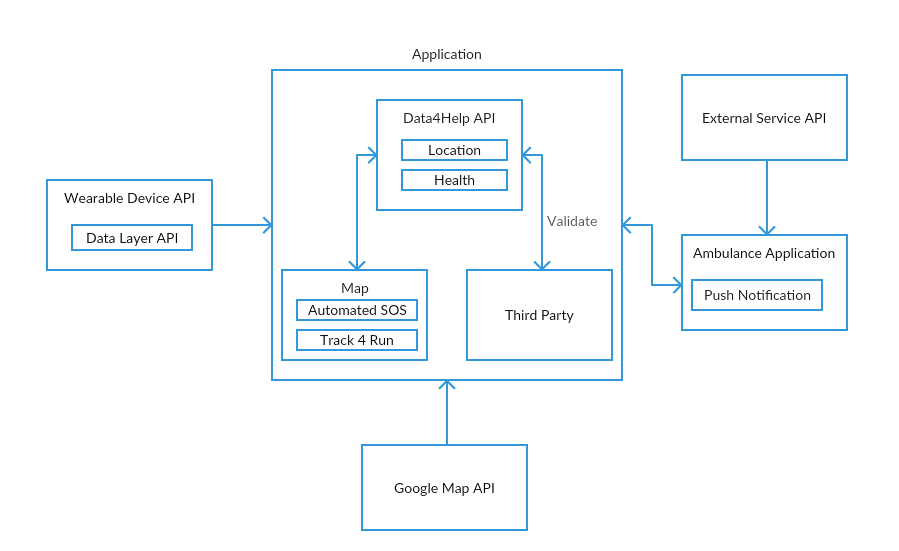
\includegraphics[width=\linewidth]		{./Diagrams/CommunicationInterface.png}
      	\caption{Communication Interface}
        \label{TrackMe_comint}
\end{figure}